\begin{enumerate}[label=\thesection.\arabic*.,ref=\thesection.\theenumi]
\numberwithin{equation}{enumi}

\item Sketch the Bode Magnitude and Phase plot for the following system. Also compute the gain margin and the phase margin.
\begin{align}
G\brak{s} &= \frac{10}{s\brak{1+0.5s}\brak{1+.01s}}
\label{eq:ee18btech11048_2}
\end{align}
\\
\solution 
The system is defined as follows:
\begin{align}
G\brak{s} &= \frac{10}{s\brak{1+0.5s}\brak{1+.01s}}
\end{align}
For the given system\\
poles = 0 , -2 , -100\\
zeros = none\\
The magnitude and phase plot are as follows: Fig  \ref{fig:ee18btech11048} 
\begin{figure}[!h]
\centering
  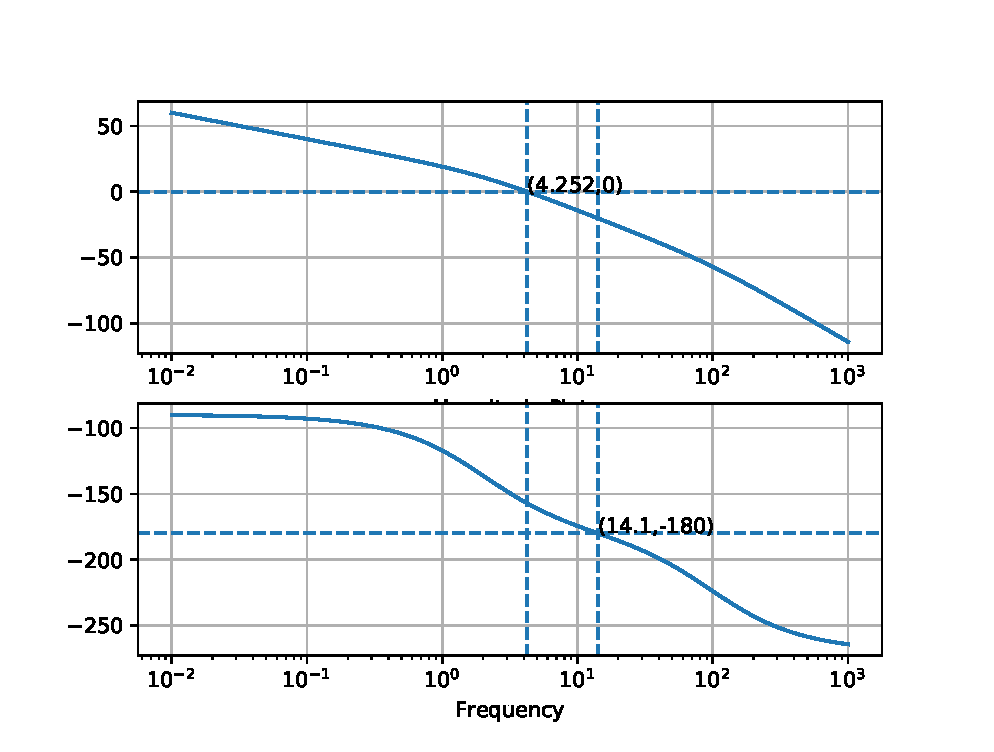
\includegraphics[width=\columnwidth]{./figs/ee18btech11048.eps}
  \caption{a}
  \label{fig:ee18btech11048}
\end{figure}

The python code to obtain the graphs:

\begin{lstlisting}
codes/ee18btech11048.py
\end{lstlisting}

\item Finding the Phase Margin\\
\begin{align}
G\brak{j\omega} &= \frac{10}{j\omega\brak{1+0.5j\omega}\brak{1+.01j\omega}}
\end{align}
{\em Phase Margin} is $\angle G(\j\omega) + 180\degree$ , where $\omega$ is frequency when gain = 1 . 
\\
\solution
\begin{align}
    \frac{100}{\omega\sqrt{\brak{0.5\omega}^2+1}\sqrt{\brak{0.01\omega}^2+1}} &= 1
\label{eq:ee18btech11048_2}
\end{align}{}
Solving \eqref{eq:ee18btech11048_2} {\em or} from Fig \ref{fig:ee18btech11048} frequency at which gain = 1 ,is gain crossover frequency $\omega_{gc}$ or where the Magnitude plot value is {\em zero}.

\begin{align}
\implies
\omega_{gc} &= 4.25  \\
\angle G\brak{\j\omega_{gc}} &= -157.2 \\
\implies
PM &= 22.8 
\end{align}

\item Finding the Gain Margin\\
{\em Gain Margin} is 0\degree $-G(\j\omega)  $ db , where $\omega_{pc}$is {\em phase crossover frequency}, frequency when phase = $-180\degree$
\\
\solution

\begin{multline}
\arctan \brak{0}-\arctan \brak{\frac{\omega}{0}} - \arctan \brak{\frac{\omega}{2}}- \\\arctan \brak{\frac{\omega}{100}} = -180\degree
\label{eq:ee18btech11048_3}
\end{multline}
Solving \eqref{eq:ee18btech11048_3} {\em or} from Fig \ref{fig:ee18btech11048}  $\omega_$ where the Phase plot value is {\em -180\degree}.

\begin{align}
\implies
\omega &=  14.1  \\
-G(\j\omega) db = -20.2 \\
\implies
GM &= 20.2 db
\end{align}

\end{enumerate}
